\cleardoublepage

\chapter{Estado de la cuestión}
\label{makereference2}

Contextualizando el entorno, la transición hacia un sistema energético descarbonizado, impulsada por la creciente penetración de fuentes de energía renovable, como la solar fotovoltaica y la eólica, presenta desafíos significativos para la estabilidad y gestión de la red eléctrica~\cite{carrasco2023battery}. Con ello, los \gls{bess} emergen como una tecnología clave para dotar de flexibilidad al sistema, solucionando el desacoplo entre la generación y el consumo de electricidad~\cite{gissey2018market}.

El mercado eléctrico, que opera usando un modelo marginalista para los mercados spot, en donde el precio es determinado mediante el cruce de la oferta y demanda, mostrado en la figura~\ref{fig:precio-casacion} extraída directamente de extraída de \gls{omie}, ofrece diversas oportunidades para los \glspl{bess}. Estas incluyen el arbitraje de energía en los mercados spot diario, intradiarios y continuo (de mayor a menor liquidez), en los que se centra el sistema desarrollado, y la participación en los servicios de ajuste~\cite{gaspar2021optimisation}, \gls{afrr} y \gls{mfrr}, donde se ofertan disponibilidades.

Por ello, la viabilidad económica depende intrínsecamente de la capacidad del sistema para formular y ejecutar estrategias de operación óptimas en un entorno de alta incertidumbre de precios y previsiones de generación~\cite{heredia2015economic}, siendo considerada incluso una ``tecnología clave para la transición energética''.

\begin{figure}
  \centering
  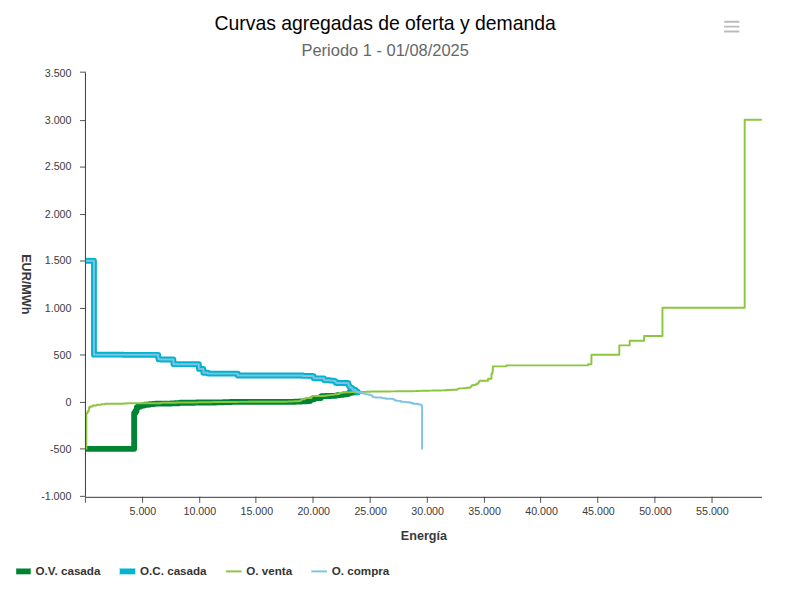
\includegraphics[width=0.6\linewidth]{figures/precio-casacion.png}
  \caption[Curva de casación del mercado eléctrico.]{Curva de casación real del inicio del mes de agosto del mercado eléctrico marginalista, donde tan solo las ofertas de compra por encima y de venta por debajo del precio de casación son aceptadas.}
  \label{fig:precio-casacion}
\end{figure}

De este modo, se analiza la situación tecnológica actual de los activos de almacenamiento desde una perspectiva de mercado multifacética en la sección~\ref{makereference2.1}, se estudian los diferentes enfoques de las estrategias de optimización concretas a lo largo de la literatura en la sección~\ref{makereference2.2}, y se detallan las soluciones comerciales existentes en relación al sistema desarrollado en la sección~\ref{makereference2.3}.

\section{Situación tecnológica}
\label{makereference2.1}

Los \glspl{bess} en los mercados eléctricos, aunque prometedores, se encuentran todavía en una fase temprana de desarrollo y adopción\footnote{Aunque no hayan sido históricamente populares en el mercado eléctrico, las baterías son usadas  gran escala en otras situaciones, como la carga de vehículos eléctricos}. Esta infancia se manifiesta en la rápida evolución de los algoritmos de optimización y en la muy notable reducción de costes de la tecnología, que son características típicas de una tecnología en las primeras etapas. Dicho fenómeno se conoce como el \textit{rate of learning} e indica que ``el coste de una tecnología disminuye a medida que aumenta su producción acumulada''~\cite{mathew2021climate, louwen2018technological}, representado en la figura~\ref{fig:rate-of-learning}.

\begin{figure}
  \centering
  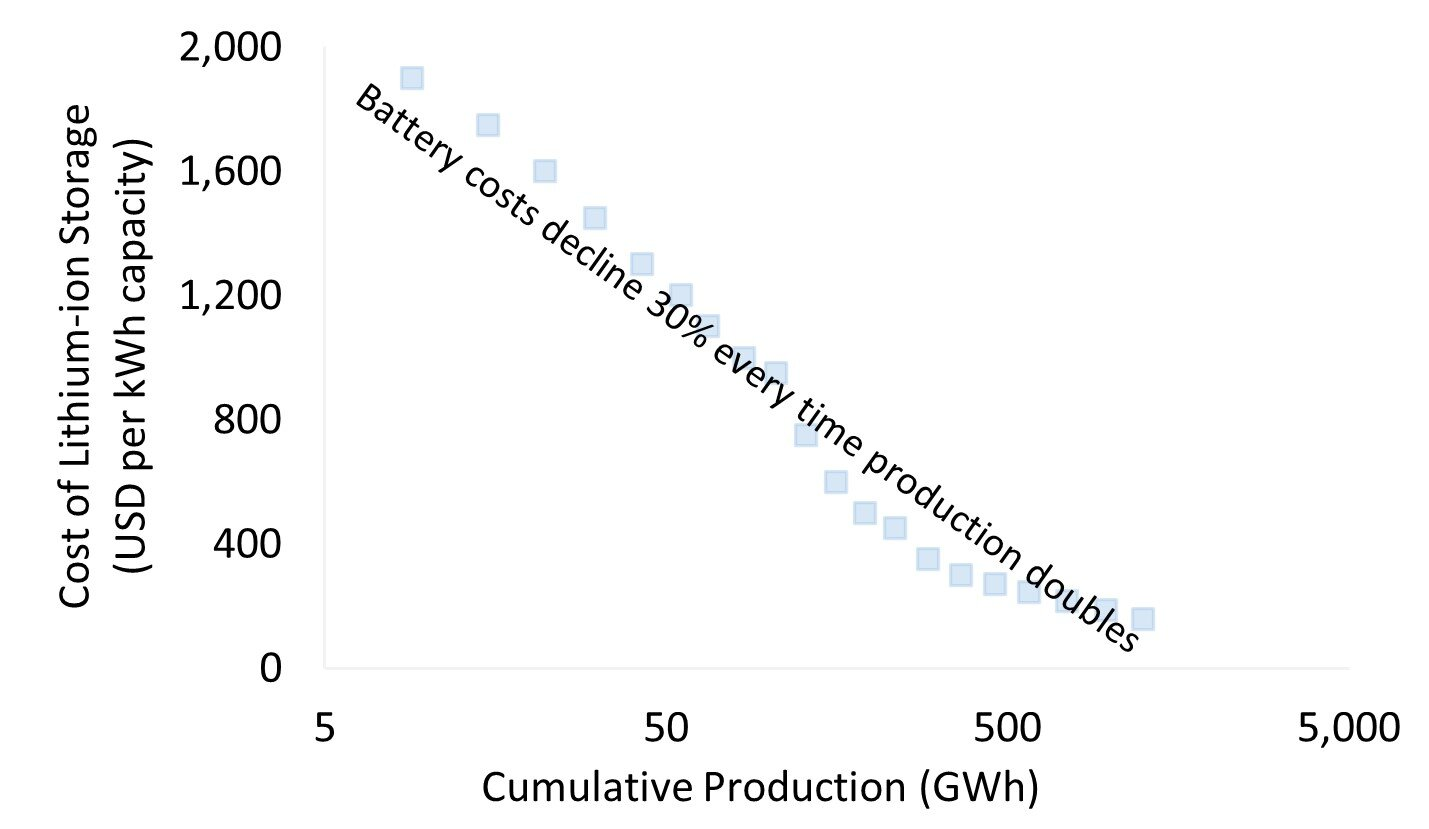
\includegraphics[width=0.75\linewidth]{figures/rate-of-learning.jpg}
  \caption[Reducción de los costes de las baterías por su uso.]{Representación de la reducción de los costes de las baterías según su uso, se observa una reducción del 10--35\% cada vez que se dobla la producción~\cite{irena2025irena}.}
  \label{fig:rate-of-learning}
\end{figure}

Por ello, la situación tecnológica de los optimizadores de \glspl{bess} varía significativamente entre el mercado eléctrico ibérico, europeo y demás, debido a diferencias en el diseño, marcos regulatorios e incentivos políticos.

Por un lado, el mercado ibérico, el pertinente al desarrollo realizado, presenta tanto oportunidades como barreras para los \glspl{bess}, y es que el altamente notorio apoyo de las tecnologías renovables crea una volatilidad de precios\footnote{Debido a la cantidad de activos solares, por ejemplo, los precios se desploman cuando hace sol, pero cuando no hay recursos renovables, los precios pueden llegar a dispararse, teniendo que hacer uso de tecnologías energéticas más caras}, que puede ser aprovechada mediante el arbitraje de energía~\cite{hu2022potential}, observado en la figura~\ref{fig:arbitraje-tecnologia}.

Sin embargo, la regulación española ha sido anteriormente considerada una de las principales barreras~\cite{hu2021barriers} con lo relacionado a las tasas energéticas (al cargar y descargar de la red), aunque la normativa evoluciona para mitigar estos problemas con grandes ayudas del estado dirigidas a las baterías, en este caso.

En la actualidad, se subraya que la producción del mercado ibérico es ínfima en comparación, figura~\ref{fig:comparacion-energia-ciclada} obtenida directamente de \gls{ree}, pero estudios económicos muestran la viabilidad potencial de los \gls{bess} si se implementa una estrategia de optimización adecuada~\cite{he2015optimal}.

\begin{figure}
  \centering
  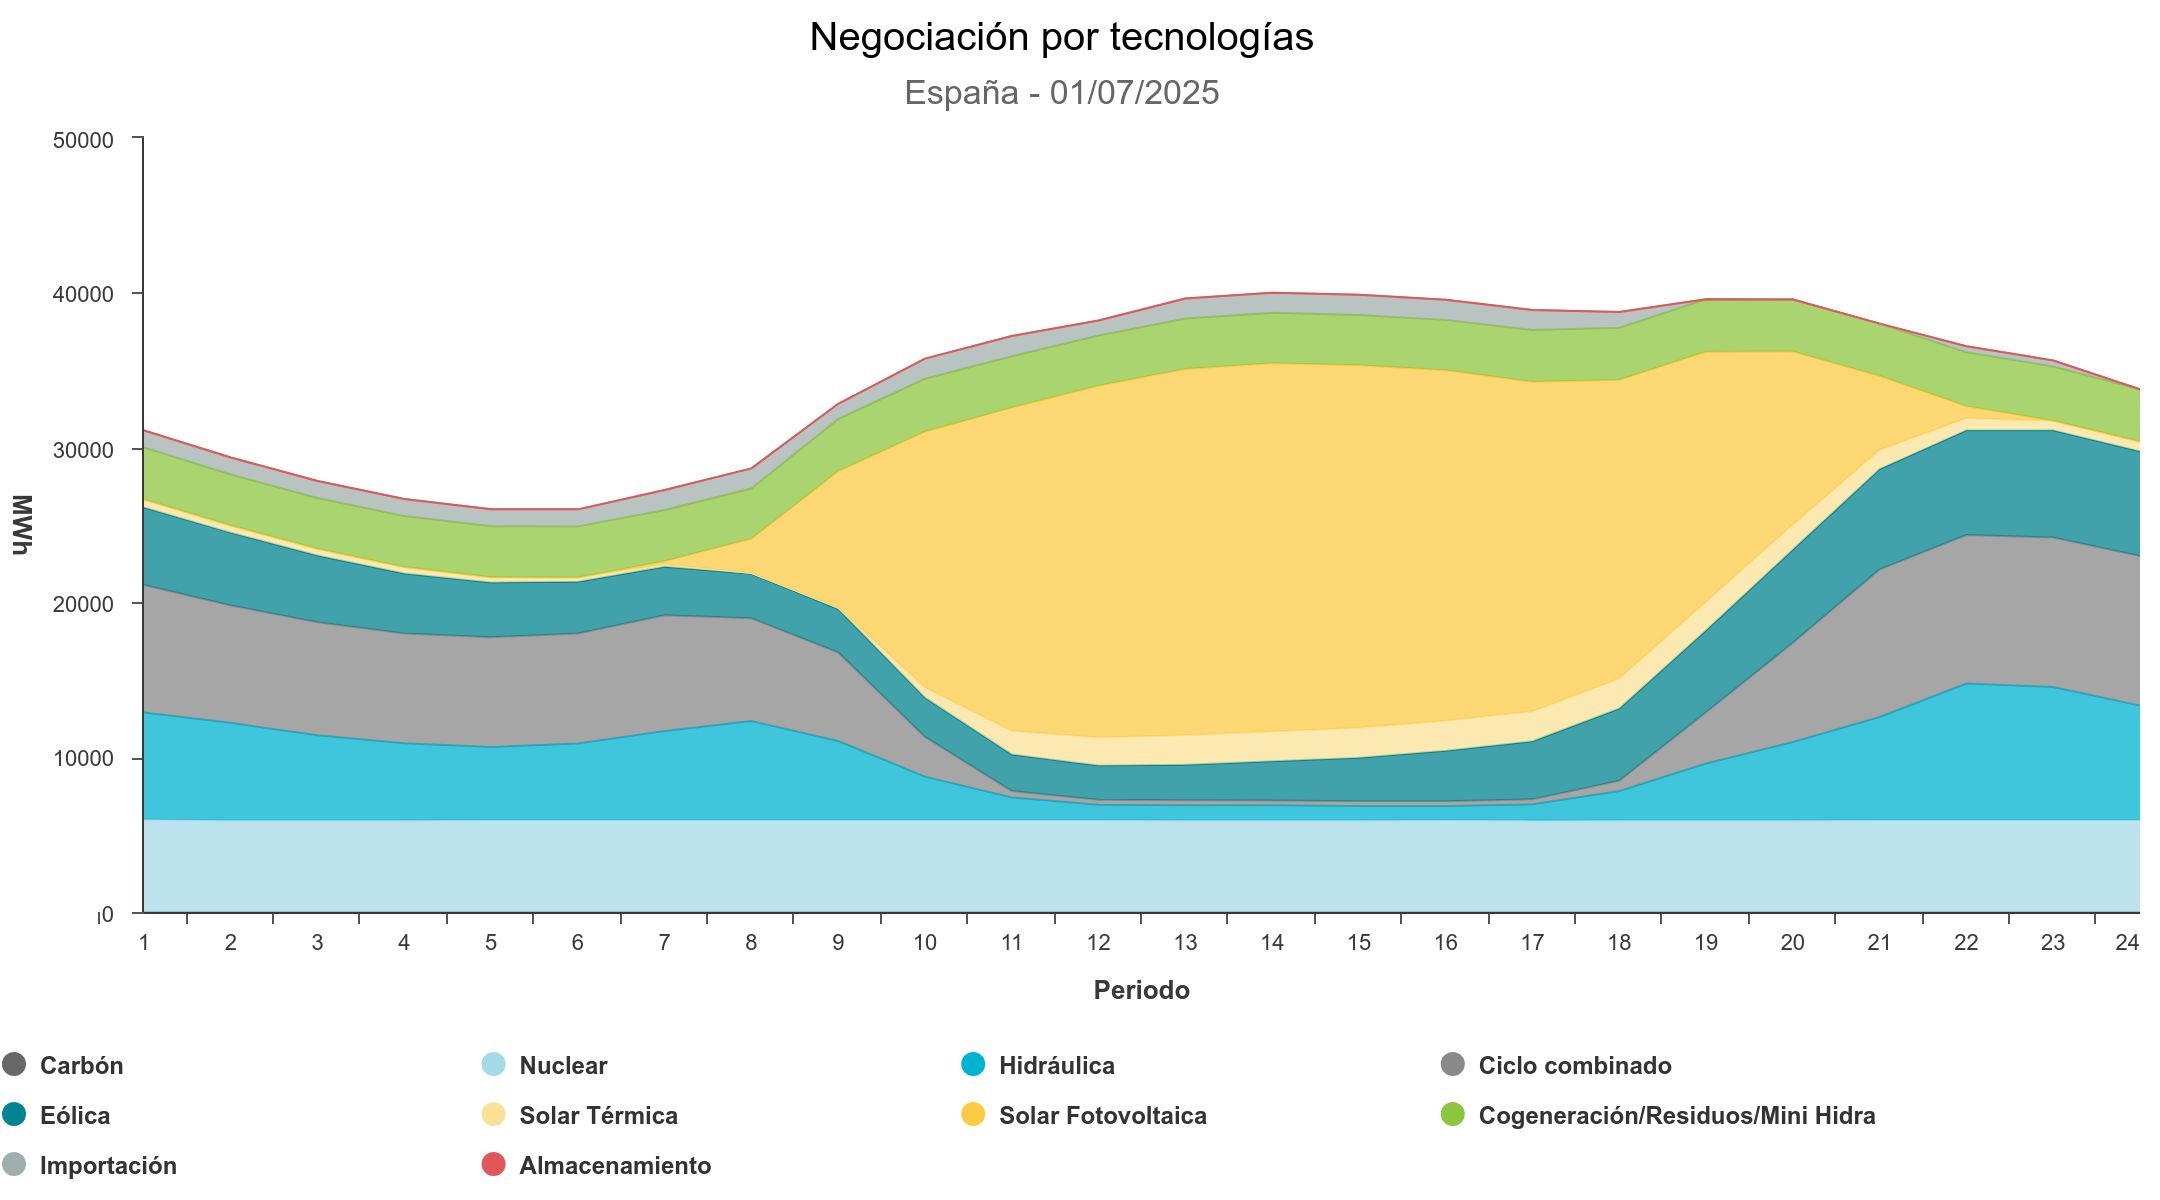
\includegraphics[width=0.75\linewidth]{figures/arbitraje-tecnologia.jpg}
  \caption[Negociación por tecnologías.]{Negociación por tecnologías del inicio del mes de junio, donde las tecnologías más caras, como el ciclo combinado, abarcan la mayor parte de la generación cuando no hay tanto recurso renovable.}
  \label{fig:arbitraje-tecnologia}
\end{figure}

\begin{figure}
  \centering
  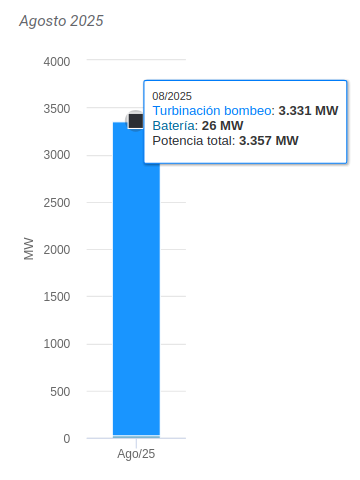
\includegraphics[width=0.4\linewidth]{figures/comparacion-energia-ciclada.png}
  \caption[Comparación de la energía diaria arbitrada.]{Comparación entre la media de la energía diaria real arbitrada durante mes de agosto entre el bombeo y las baterías, negociadas públicamente por el sistema desarrollado.}
  \label{fig:comparacion-energia-ciclada}
\end{figure}

A nivel europeo, países como Alemania y Reino Unido han sido los pioneros en la integración de \glspl{bess}~\cite{kivipelto2017grid, tejada2019review}, principalmente a través de mercados de regulación de frecuencia desorbitadamente remunerados, aunque la saturación de estos mercados este llevando a una mayor dependencia de los ingresos del arbitraje de energía en los mercados spot (relacionados con el trabajo realizado).

De esta forma, los mercados europeos encaminan la situación futura del mercado ibérico, como se ve reflejado en la actualidad~\cite{kumar2019strategic}.

\section{Estrategias de optimización}
\label{makereference2.2}

Aunque irónicamente el panorama de los \glspl{bess} en los mercados pertinentes estuviera prácticamente desierto antes de la incursión del sistema desarrollado, la literatura científica describe una variedad de enfoques de estrategias de optimización, desde la programación matemática hasta el uso de la propia inteligencia artificial.

Se observa que los modelos de programación matemática, de \gls{lp} y \gls{milp}, son los más comúnmente utilizados para la optimización de \glspl{bess}. Estos modelos buscan maximizar una o varias funciones objetivo (generalmente el beneficio económico) sujetas a un conjunto de restricciones que representan la situación física de la batería y las reglas del mercado~\cite{mendoza2023review}. La principal ventaja de estos métodos, y la razón de su uso en el desarrollo, es su capacidad para encontrar una solución óptima garantizada.

Precisamente, la tendencia en alza de estas estrategias es la incorporación del modelado de la degradación en la formulación del sistema~\cite{liu2022milp, minh2024mixed, spiller2020aging}, intrínsecamente favoreciendo la estabilidad a largo plazo, principalmente centradas en la configuración topológica híbrida.

Interesanetemente, con la creciente complejidad de los mercados y la necesidad de adaptarse a condiciones cambiantes, técnicas de inteligencia artificial han comenzado a ser investigadas~\cite{haratian2024machine, krishna2024advanced}. Resulta que algoritmos de aprendizaje por refuerzo son particularmente prometedores~\cite{dong2021strategic}, ya que permiten a un agente aprender la estrategia de operación óptima a través de la interacción directa con el entorno del mercado, sin necesidad de un modelo matemático perfecto, aunque soluciones combinando los dos aspectos hayan sido propuestas~\cite{georgiadis2025hybrid}. Estos métodos son capaces de manejar la incertidumbre y la dinámica estocástica (aleatoria) de los precios del mercado de manera más robusta que los métodos tradicionales.

Incluso existen esfuerzos realizados al respecto dentro del contexto del mercado ibérico, como los centros técnológicos enfocados en el desarrollo de \glspl{bms} a través de tecnologías más heterodoxas~\cite{ikerlan2025bateria}.

\section{Soluciones comerciales}
\label{makereference2.3}

Empresas extranjeras fuera del mercado iberico, como Enspired~\cite{enspired2025battery} en Austria, Entelios~\cite{entelios2025cross} en Alemania y Sympower~\cite{sympower2025battery} en Países Bajos, se especializan en la comercialización y optimización de activos energéticos, incluyendo los \glspl{bess}. Precisamente, más allá de la literatura, las soluciones comerciales, al igual que el trabajo realizado, son capaces de ofrecer una visión integral de todos los aspectos relacionados con la optimización de baterías, desde la infraestructura operacional, el entorno de mercado, la modelización estructural y la consigna y control.

Aunque sus estrategias de mercado sean propietarias, su operación se basa en los principios de licitación conocidos y, en este caso, en la participación en múltiples mercados, tanto spot como de regulación, para apilar los flujos de ingresos, realizando el llamado \textit{revenue stacking}~\cite{rancilio2022revenue}.

De esta forma, en caso de ser compatibles con el mercado ibérico, el \textit{revenue stacking} se considera la ventaja principal de los sistemas de optimización de baterías en el mercado eléctrico comerciales ya asentados, con respecto al trabajo realizado.
